\chapter{Langevin Dynamics and Fokker-Planck Equations}
\label{ch:langevin}

\section{The Physical Intuition of Generative Diffusion}

The previous chapter introduced score-based generative modeling as a mechanism for learning the gradient fields of data distributions. While the empirical success of mapping noise to data via score functions is undeniable, a rigorous mathematical framework is required to formalize this process. To build this foundation, we turn to non-equilibrium statistical mechanics, specifically the study of particles suspended in a fluid subject to thermal fluctuations.

In physics, the macroscopic behavior of a diffusing substance (like a drop of ink in water) is fundamentally connected to the microscopic, erratic trajectories of individual particles. The mathematician Paul Langevin described the microscopic perspective by modeling the motion of a single particle under the influence of two competing forces: a deterministic drift pushing the particle down a potential energy gradient, and a stochastic diffusion caused by random collisions with fluid molecules. The continuous-time stochastic process describing this particle's trajectory is known as \emph{Langevin dynamics}.

When we transpose this physical model into the realm of deep generative learning, the "particle" becomes a single data point navigating a high-dimensional space $\mathcal{X}$. The "potential energy landscape" is defined by the negative log-likelihood of our data distribution, $U(x) = -\log p_{\text{data}}(x)$. The deterministic drift force pulling the particle toward regions of low energy is therefore precisely the score function: $-\nabla U(x) = \nabla \log p_{\text{data}}(x)$. This drift continuously pulls the state toward the high-density manifolds of the data. 

Simultaneously, the "thermal noise" injected into the system acts as an exploratory force. Without noise, particles would deterministically fall into the nearest local maximum of the data density and halt, resulting in mode collapse. The continuous injection of Brownian noise prevents the particle from becoming permanently trapped in spurious local optima, ensuring that the system explores the entire state space and samples from the global probability distribution in exact proportion to $p_{\text{data}}(x)$.

While Langevin dynamics characterizes the microscopic path of a single point $X_t$, it is often more illuminating to track the macroscopic evolution of an entire ensemble of particles. If we initialize a cloud of particles from an arbitrary prior distribution and let each undergo independent Langevin dynamics, how does the probability density of the cloud, $p_t(x)$, evolve over time? The deterministic partial differential equation governing this evolving density is the \emph{Fokker-Planck equation} (also known in probability theory as the Kolmogorov forward equation). 

The Fokker-Planck equation is the bridge between the microscopic stochasticity of data generation and the macroscopic determinism of probability distributions. By leveraging this equation, we can mathematically prove that the stationary state of Langevin dynamics is exactly the true data distribution. Furthermore, from an information-theoretic perspective, we can demonstrate that the entropy of the system evolves in a strictly monotonic fashion, continuously dissipating the Kullback-Leibler divergence between the current distribution and the target data distribution. In this chapter, we formalize these dynamics and establish the continuous-time backbone upon which modern diffusion models operate.

\section{Mathematical Primer: Measure Theory and It\^o Calculus}

The transition from discrete Markov chains to continuous-time stochastic processes requires a fundamental shift in our mathematical toolkit. In discrete time, a random walk is easily understood as a sequence of random variables. However, if we attempt to take the continuous-time limit by shrinking the step size to zero while maintaining a finite variance, the resulting trajectories exhibit pathological behavior: they become continuous everywhere but differentiable nowhere. 

To formalize such processes, we cannot rely on standard Riemann calculus. Instead, we must turn to measure theory and It\^o calculus. Measure theory provides the rigorous foundation for defining probabilities over uncountably infinite dimensional path spaces. The central object of this theory for our purposes is the Wiener measure, which formalizes the distribution of standard Brownian motion.

\begin{definition}[Standard Brownian Motion]
A standard $d$-dimensional Brownian motion, or Wiener process, is a continuous-time stochastic process $\{W_t\}_{t \ge 0}$ characterized by three properties:
\begin{enumerate}
    \item $W_0 = 0$ almost surely.
    \item For any $0 \le s < t$, the increment $W_t - W_s$ is independent of the past values $W_u$ for all $0 \le u \le s$.
    \item The increments are normally distributed: $W_t - W_s \sim \mathcal{N}(0, (t-s)I)$.
\end{enumerate}
\end{definition}

Because the increments of Brownian motion scale with $\sqrt{\Delta t}$ rather than $\Delta t$, the quadratic variation of $W_t$ over a time interval is non-zero. Consequently, the standard rules of classical calculus fail. If we apply a smooth nonlinear function to a stochastic process, the traditional chain rule does not hold. 

To analyze the temporal evolution of such systems, we must use It\^o calculus, which extends classical calculus by incorporating the second-order effects of stochastic fluctuations. 

\begin{lemma}[It\^o's Lemma]
Let $X_t$ be a $d$-dimensional It\^o process governed by the stochastic differential equation $dX_t = \mu(X_t, t) dt + \sigma(X_t, t) dW_t$. For any twice continuously differentiable function $f(x, t) : \mathbb{R}^d \times \mathbb{R} \to \mathbb{R}$, the differential of $f(X_t, t)$ is given by:
\begin{equation}
    df = \left( \frac{\partial f}{\partial t} + \nabla_x f^\top \mu + \frac{1}{2} \text{Tr}\left( \sigma \sigma^\top \nabla^2_x f \right) \right) dt + \nabla_x f^\top \sigma \, dW_t
\end{equation}
\end{lemma}

The crucial addition in It\^o's Lemma is the second-order trace term involving the Hessian $\nabla^2_x f$. This term captures the macroscopic drift generated by the accumulation of microscopic variance. With these mathematical tools established, we can now rigorously define our continuous-time generative dynamics.

\section{Langevin Dynamics and Stochastic Differential Equations}

We begin by formally defining the continuous-time process. Let $X_t \in \mathbb{R}^d$ be a random variable representing the state of our generative process at time $t \ge 0$. The evolution of $X_t$ is governed by a Stochastic Differential Equation (SDE) of the form:

\begin{equation}
    dX_t = \mu(X_t, t) dt + \sigma(X_t, t) dW_t
\end{equation}

where $\mu: \mathbb{R}^d \times \mathbb{R} \to \mathbb{R}^d$ is the drift coefficient, $\sigma: \mathbb{R}^d \times \mathbb{R} \to \mathbb{R}^{d \times d}$ is the diffusion coefficient, and $W_t$ is a standard $d$-dimensional Brownian motion (or Wiener process). The Wiener process formally represents the continuous-time limit of a random walk, characterized by continuous paths and independent, normally distributed increments $W_{t+\Delta t} - W_t \sim \mathcal{N}(0, \Delta t I)$.

\begin{definition}[Overdamped Langevin Dynamics]
Let $p_{\text{data}}(x)$ be a continuously differentiable target probability density on $\mathbb{R}^d$. The \emph{overdamped Langevin dynamics} associated with $p_{\text{data}}$ is the SDE given by:
\begin{equation}
    dX_t = \nabla \log p_{\text{data}}(X_t) dt + \sqrt{2} dW_t
\end{equation}
\end{definition}

In this specific SDE, the drift term is the score function $\mu(X_t, t) = \nabla \log p_{\text{data}}(X_t)$, which points in the direction of steepest ascent in the data density. The diffusion matrix is constant, $\sigma(X_t, t) = \sqrt{2} I$. The constant $\sqrt{2}$ is carefully chosen to balance the deterministic drift and the stochastic noise such that the system ultimately converges to $p_{\text{data}}(x)$.

\begin{figure}[htpb]
\centering
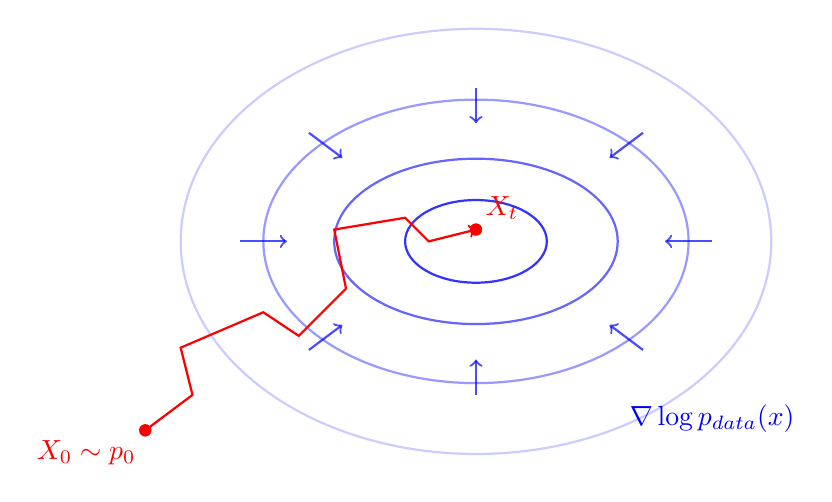
\begin{tikzpicture}[scale=1.5]
  % Contours representing the data distribution density
  \draw[thick, blue!20] (0,0) ellipse (2.5cm and 1.8cm);
  \draw[thick, blue!40] (0,0) ellipse (1.8cm and 1.2cm);
  \draw[thick, blue!60] (0,0) ellipse (1.2cm and 0.7cm);
  \draw[thick, blue!80] (0,0) ellipse (0.6cm and 0.35cm);
  
  \node[blue] at (2.0, -1.5) {$\nabla \log p_{\text{data}}(x)$};
  
  % Vector field arrows representing the score (drift)
  \foreach \angle in {0, 45, 90, 135, 180, 225, 270, 315} {
    \draw[->, blue, thick, opacity=0.7] (\angle:2.0cm and 1.3cm) -- (\angle:1.6cm and 1.0cm);
  }
  
  % Langevin Trajectory
  \draw[red, thick, ->] (-2.8, -1.6) 
    -- (-2.4, -1.3) -- (-2.5, -0.9) -- (-1.8, -0.6) 
    -- (-1.5, -0.8) -- (-1.1, -0.4) -- (-1.2, 0.1) 
    -- (-0.6, 0.2) -- (-0.4, 0.0) -- (0.0, 0.1);
  
  \fill[red] (-2.8, -1.6) circle (1.5pt) node[below left] {$X_0 \sim p_0$};
  \fill[red] (0.0, 0.1) circle (1.5pt) node[above right] {$X_t$};
\end{tikzpicture}
\caption{A simulated microscopic trajectory of Langevin dynamics. The particle $X_t$ starts from an initial prior distribution and performs a random walk biased by the score function (blue arrows) toward the high-density regions of $p_{\text{data}}(x)$.}
\label{fig:langevin_trajectory}
\end{figure}


\section{The Fokker-Planck Equation}

To understand how the probability density $p_t(x)$ of the random variable $X_t$ evolves over time, we transition from the microscopic SDE to the macroscopic partial differential equation. 

For a general It\^o SDE $dX_t = \mu(X_t, t) dt + \sigma(X_t, t) dW_t$, the evolution of its marginal probability density function $p_t(x)$ is deterministically governed by the Fokker-Planck equation:
\begin{equation}
    \frac{\partial p_t(x)}{\partial t} = -\sum_{i=1}^d \frac{\partial}{\partial x_i} \left[ \mu_i(x, t) p_t(x) \right] + \frac{1}{2} \sum_{i=1}^d \sum_{j=1}^d \frac{\partial^2}{\partial x_i \partial x_j} \left[ (\sigma(x,t) \sigma(x,t)^\top)_{ij} p_t(x) \right]
\end{equation}
Substituting the specific coefficients for our Langevin dynamics, $\mu(x, t) = \nabla \log p_{\text{data}}(x)$ and $\sigma(x, t) = \sqrt{2} I$, the second-order diffusion tensor becomes $(\sqrt{2} I)(\sqrt{2} I)^\top = 2I$. This simplifies the Fokker-Planck equation to:

\begin{equation}
    \label{eq:langevin_fpe}
    \frac{\partial p_t(x)}{\partial t} = -\nabla \cdot \left( p_t(x) \nabla \log p_{\text{data}}(x) \right) + \Delta p_t(x)
\end{equation}

where $\nabla \cdot (\cdot)$ denotes the divergence operator and $\Delta = \nabla \cdot \nabla$ is the Laplace operator. The first term on the right-hand side represents the advection of the probability mass driven by the score field, effectively concentrating density in modes. The second term, the Laplacian, represents isotropic heat diffusion, effectively smoothing and spreading the probability mass.

\begin{figure}[htpb]
\centering
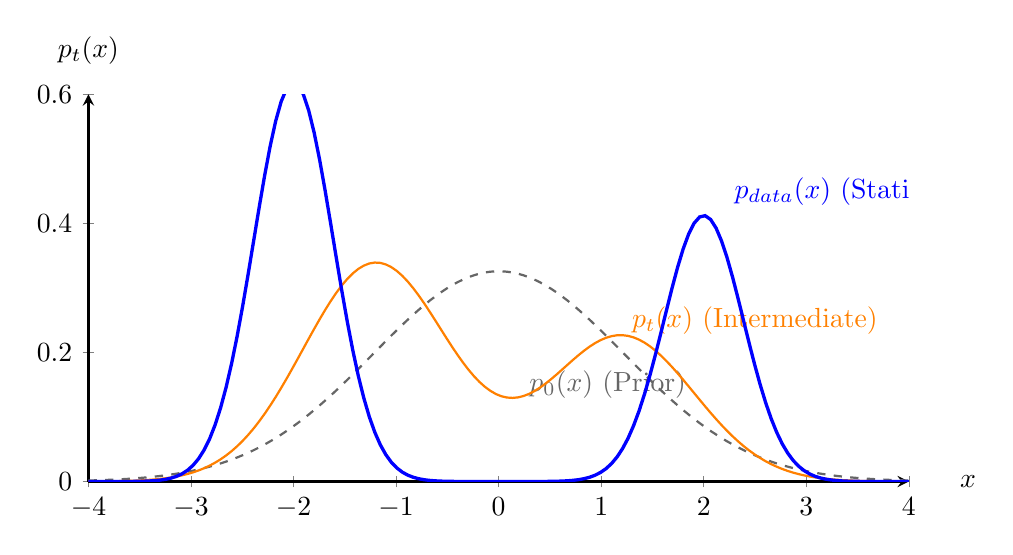
\begin{tikzpicture}
  \begin{axis}[
      width=12cm, height=6.5cm,
      xlabel=$x$, ylabel={$p_t(x)$},
      domain=-4:4,
      samples=150,
      axis lines=left,
      every axis y label/.style={at={(axis description cs:0,1.05)},anchor=south},
      every axis x label/.style={at={(axis description cs:1.05,0)},anchor=west},
      no marks,
      thick,
      ymax=0.6,
      ymin=0
    ]
    
    % Initial distribution (Prior)
    \addplot[black!60, dashed, thick] {1/(sqrt(2*pi*1.5)) * exp(-x^2/(2*1.5))};
    \node[black!60, right] at (axis cs:0.2, 0.15) {$p_0(x)$ (Prior)};
    
    % Intermediate distribution
    \addplot[orange, thick] {0.4 * 1/(sqrt(2*pi*0.5)) * exp(-(x-1.2)^2/(2*0.5)) + 0.6 * 1/(sqrt(2*pi*0.5)) * exp(-(x+1.2)^2/(2*0.5))};
    \node[orange, right] at (axis cs:1.2, 0.25) {$p_t(x)$ (Intermediate)};
    
    % Target distribution (bimodal)
    \addplot[blue, very thick] {0.4 * 1/(sqrt(2*pi*0.15)) * exp(-(x-2)^2/(2*0.15)) + 0.6 * 1/(sqrt(2*pi*0.15)) * exp(-(x+2)^2/(2*0.15))};
    \node[blue, right] at (axis cs:2.2, 0.45) {$p_{\text{data}}(x)$ (Stationary)};

  \end{axis}
\end{tikzpicture}
\caption{Macroscopic evolution of the probability density according to the Fokker-Planck equation. An initially broad prior density $p_0(x)$ is simultaneously transported and shaped by the score function until it exactly matches the multi-modal stationary target distribution $p_{\text{data}}(x)$.}
\label{fig:fokker_planck_evolution}
\end{figure}

\section{Stationarity of the Data Distribution}

The fundamental reason we employ Langevin dynamics in generative modeling is that its equilibrium state perfectly reconstructs the unknown data distribution. We can rigorously prove this by finding the stationary solution to the Fokker-Planck equation.

\begin{theorem}[Stationary Distribution of Langevin Dynamics]
\label{thm:langevin_stationarity}
Let $p_{\text{data}}(x)$ be a probability density on $\mathbb{R}^d$. If $X_t$ evolves according to the Langevin dynamics $dX_t = \nabla \log p_{\text{data}}(X_t) dt + \sqrt{2} dW_t$, then $p_{\text{data}}(x)$ is a stationary distribution of the process.
\end{theorem}

\begin{proof}
A distribution is stationary if, when the process reaches it, the density no longer changes over time. Mathematically, this requires $\frac{\partial p_t(x)}{\partial t} = 0$. We substitute $p_t(x) = p_{\text{data}}(x)$ into the right-hand side of the Fokker-Planck Equation \eqref{eq:langevin_fpe}:
\begin{align*}
    \frac{\partial p_t(x)}{\partial t} &= -\nabla \cdot \left( p_{\text{data}}(x) \nabla \log p_{\text{data}}(x) \right) + \Delta p_{\text{data}}(x)
\end{align*}
Recall the logarithmic derivative identity: $\nabla p(x) = p(x) \nabla \log p(x)$. Using this identity, we rewrite the advection term:
\begin{align*}
    p_{\text{data}}(x) \nabla \log p_{\text{data}}(x) &= \nabla p_{\text{data}}(x)
\end{align*}
Substituting this back into the divergence operator yields:
\begin{align*}
    \frac{\partial p_t(x)}{\partial t} &= -\nabla \cdot \left( \nabla p_{\text{data}}(x) \right) + \Delta p_{\text{data}}(x) \\
    &= -\Delta p_{\text{data}}(x) + \Delta p_{\text{data}}(x) \\
    &= 0
\end{align*}
Because the time derivative vanishes everywhere, $p_{\text{data}}(x)$ is an invariant measure of the stochastic differential equation.
\end{proof}

\section{Information-Theoretic Convergence: The H-Theorem}

Theorem \ref{thm:langevin_stationarity} proves that if the process reaches $p_{\text{data}}$, it stays there. But does it actually converge to $p_{\text{data}}$ from an arbitrary prior distribution? We can prove convergence by tracking the Kullback-Leibler (KL) divergence $D_{\text{KL}}(p_t \parallel p_{\text{data}})$. This analysis yields a continuous-time analog to the Second Law of Thermodynamics (often referred to as an H-theorem or a generalized de Bruijn's identity).

\begin{theorem}[Monotonic Dissipation of KL Divergence]
\label{thm:kl_dissipation}
Let $p_t(x)$ be the probability density of the state $X_t$ under the Langevin dynamics associated with $p_{\text{data}}(x)$. Assuming suitable regularity conditions such that integration by parts holds and boundary terms vanish at infinity, the KL divergence between $p_t$ and $p_{\text{data}}$ is monotonically non-increasing:
\begin{equation}
    \frac{d}{dt} D_{\text{KL}}(p_t \parallel p_{\text{data}}) \le 0
\end{equation}
\end{theorem}

\begin{proof}
By definition, the KL divergence is:
\begin{align*}
    D_{\text{KL}}(p_t \parallel p_{\text{data}}) &= \int p_t(x) \log \frac{p_t(x)}{p_{\text{data}}(x)} dx
\end{align*}
Taking the time derivative, we apply the Leibniz integral rule:
\begin{align}
    \frac{d}{dt} D_{\text{KL}}(p_t \parallel p_{\text{data}}) &= \int \frac{\partial p_t}{\partial t} \log \frac{p_t}{p_{\text{data}}} dx + \int p_t \frac{\partial}{\partial t} \left( \log p_t - \log p_{\text{data}} \right) dx \nonumber \\
    &= \int \frac{\partial p_t}{\partial t} \log \frac{p_t}{p_{\text{data}}} dx + \int p_t \left( \frac{1}{p_t} \frac{\partial p_t}{\partial t} \right) dx \nonumber \\
    &= \int \frac{\partial p_t}{\partial t} \log \frac{p_t}{p_{\text{data}}} dx + \frac{d}{dt} \int p_t dx \label{eq:kl_deriv}
\end{align}
Because $p_t(x)$ is a valid probability density for all $t$, $\int p_t dx = 1$, making its time derivative zero. We now substitute the Fokker-Planck equation for $\frac{\partial p_t}{\partial t}$. First, we rewrite the FPE in a more convenient form:
\begin{align*}
    \frac{\partial p_t}{\partial t} &= -\nabla \cdot \left( p_t \nabla \log p_{\text{data}} \right) + \nabla \cdot \left( \nabla p_t \right) \\
    &= \nabla \cdot \left( p_t \nabla \log p_t - p_t \nabla \log p_{\text{data}} \right) \\
    &= \nabla \cdot \left( p_t \nabla \log \frac{p_t}{p_{\text{data}}} \right)
\end{align*}
Substituting this back into Equation \eqref{eq:kl_deriv} yields:
\begin{equation*}
    \frac{d}{dt} D_{\text{KL}}(p_t \parallel p_{\text{data}}) = \int \nabla \cdot \left( p_t \nabla \log \frac{p_t}{p_{\text{data}}} \right) \log \frac{p_t}{p_{\text{data}}} dx
\end{equation*}
We now apply multivariate integration by parts (Green's first identity). Assuming the density decays sufficiently fast at infinity, the boundary terms evaluate to zero:
\begin{align*}
    \frac{d}{dt} D_{\text{KL}}(p_t \parallel p_{\text{data}}) &= -\int p_t(x) \left( \nabla \log \frac{p_t(x)}{p_{\text{data}}(x)} \right) \cdot \left( \nabla \log \frac{p_t(x)}{p_{\text{data}}(x)} \right) dx \\
    &= -\int p_t(x) \left\| \nabla \log \frac{p_t(x)}{p_{\text{data}}(x)} \right\|_2^2 dx \\
    &= -\mathbb{E}_{X \sim p_t} \left[ \left\| \nabla \log p_t(X) - \nabla \log p_{\text{data}}(X) \right\|_2^2 \right] \le 0
\end{align*}
This completes the proof. The quantity on the right is exactly the negative \emph{relative Fisher information}. Because it is an expectation of a squared norm, it is strictly non-positive, ensuring that the process irreversibly consumes information until it converges exactly to the target distribution.
\end{proof}


\section{Numerical Example: Discretization Bias}

In practice, a neural network is trained to approximate the score $\nabla \log p_{\text{data}}(x)$, and the continuous-time SDE must be discretized for computer simulation. The most common discretization is the Euler-Maruyama method, which yields the Unadjusted Langevin Algorithm (ULA). For a step size $\epsilon > 0$, the update rule is:
\begin{equation}
    x_{k+1} = x_k + \epsilon \nabla \log p_{\text{data}}(x_k) + \sqrt{2\epsilon} z_k, \quad z_k \sim \mathcal{N}(0, I)
\end{equation}
While continuous Langevin dynamics perfectly matches $p_{\text{data}}$, the discrete-time approximation introduces a fundamental \emph{discretization bias}. We can compute this bias exactly for a simple Gaussian target.

Suppose the data distribution is a zero-mean Gaussian with variance $\sigma^2$: $p_{\text{data}}(x) = \mathcal{N}(0, \sigma^2)$. The exact score is $\nabla \log p_{\text{data}}(x) = -x / \sigma^2$. The ULA update becomes:
\begin{equation}
    x_{k+1} = x_k - \epsilon \frac{x_k}{\sigma^2} + \sqrt{2\epsilon} z_k = \left( 1 - \frac{\epsilon}{\sigma^2} \right) x_k + \sqrt{2\epsilon} z_k
\end{equation}
This is a first-order autoregressive AR(1) process. Taking the variance of both sides and assuming independence between $x_k$ and the noise $z_k$:
\begin{equation}
    \text{Var}(x_{k+1}) = \left( 1 - \frac{\epsilon}{\sigma^2} \right)^2 \text{Var}(x_k) + 2\epsilon \text{Var}(z_k)
\end{equation}
At equilibrium (stationarity), $\text{Var}(x_{k+1}) = \text{Var}(x_k) = v_\infty$. Solving for $v_\infty$:
\begin{align*}
    v_\infty &= \left( 1 - \frac{2\epsilon}{\sigma^2} + \frac{\epsilon^2}{\sigma^4} \right) v_\infty + 2\epsilon \\
    v_\infty \left( \frac{2\epsilon}{\sigma^2} - \frac{\epsilon^2}{\sigma^4} \right) &= 2\epsilon \\
    v_\infty &= \frac{2\epsilon}{\frac{2\epsilon}{\sigma^2} - \frac{\epsilon^2}{\sigma^4}} = \frac{2\sigma^4}{2\sigma^2 - \epsilon} = \sigma^2 \left( \frac{1}{1 - \frac{\epsilon}{2\sigma^2}} \right)
\end{align*}
For a strictly positive step size $\epsilon > 0$ (specifically, $\epsilon < 2\sigma^2$ for stability), the stationary variance $v_\infty$ is strictly greater than the target variance $\sigma^2$. Using a Taylor expansion for small $\epsilon$, $v_\infty \approx \sigma^2 + \frac{\epsilon}{2}$. 

This analysis reveals a stark reality: numerical simulation of Langevin dynamics systematically over-disperses the sampled distribution. In deep generative modeling, this bias manifests as blurry or noisy samples if the step size $\epsilon$ is not carefully annealed to zero over the course of sampling.

\begin{horizon}
The mathematical elegance of Langevin dynamics relies intrinsically on the injection of stochastic noise. However, one of the most remarkable realizations in recent diffusion research is that the \emph{marginal densities} $p_t(x)$ prescribed by the Fokker-Planck equation can be achieved via entirely deterministic trajectories. It is conjectured that for any stochastic differential equation, there exists a corresponding deterministic ordinary differential equation (a Probability Flow ODE) whose continuous-time evolution traces the exact same sequence of marginal distributions, mapping the prior to the data distribution without ever explicitly injecting noise. 

An open question is whether these Probability Flow ODEs can be conceptualized as optimal transport maps, minimizing a specific dynamic cost function (such as the Wasserstein distance) between the prior and data manifolds. Future work might show that instead of simulating thousands of discrete Langevin steps, we can directly regress the vector field of this optimal transport map, effectively "rectifying" the generative flow into a straight line. 

Furthermore, while our derivation assumes a flat Euclidean space $\mathbb{R}^d$, real-world data (such as molecular conformations or climate systems) frequently resides on non-Euclidean manifolds. Extending the Fokker-Planck equation to Riemannian manifolds requires substituting the standard Laplacian with the Laplace-Beltrami operator. It is conjectured that formulating score-matching and Langevin dynamics intrinsically in the geometric space of the data will drastically reduce the discretization bias observed in current models, paving the way for generative physics simulations.
\end{horizon}

\section*{Chapter Summary}
\begin{itemize}
    \item \textbf{Langevin Dynamics:} An SDE that models microscopic particle trajectories, driven by the score function $\nabla \log p_{\text{data}}(x)$ as a deterministic drift, counterbalanced by continuous Brownian motion.
    \item \textbf{The Fokker-Planck Equation:} A deterministic PDE that describes the macroscopic time-evolution of the probability density $p_t(x)$ of particles undergoing an SDE.
    \item \textbf{Stationarity:} The data distribution $p_{\text{data}}(x)$ is analytically proven to be the exact stationary solution to the Fokker-Planck equation for Langevin dynamics.
    \item \textbf{KL Dissipation:} As the dynamics unfold, the Kullback-Leibler divergence between the current density and the data density decreases monotonically, driven by the relative Fisher information.
    \item \textbf{Discretization Bias:} In practice, discrete-time integration (like the Euler-Maruyama method) prevents perfect convergence, resulting in a stationary distribution with artificially inflated variance unless the step size approaches zero.
\end{itemize}

\section*{Exercises}
\begin{enumerate}
    \item \textbf{The Ornstein-Uhlenbeck Process:} Consider the SDE $dX_t = -\theta X_t dt + \sigma dW_t$ for $\theta, \sigma > 0$. Write down the corresponding Fokker-Planck equation. Solve for the stationary density by setting $\frac{\partial p_t(x)}{\partial t} = 0$ and integrating. Show that the stationary distribution is Gaussian and find its mean and variance.
    \item \textbf{Metropolis-Adjusted Langevin Algorithm (MALA):} Explain how adding an accept/reject step based on the Metropolis-Hastings criterion to the ULA updates eliminates the $\mathcal{O}(\epsilon)$ discretization bias derived in the numerical example. What is the acceptance probability formula?
    \item \textbf{Score Matching Objective:} Prove that minimizing the relative Fisher information $\mathbb{E}_{X \sim p_t}[\| \nabla \log p_t(X) - s_\theta(X) \|^2]$ with respect to a neural network $s_\theta$ is equivalent (up to a constant independent of $\theta$) to minimizing the explicit score matching objective $\mathbb{E}_{X \sim p_t}[\| \nabla \log p_{\text{data}}(X) - s_\theta(X) \|^2]$. Why is this identity practically useful?
\end{enumerate}

% TODO-CITE: Ensure all named results are cited.
